\subsubsection{步兵机器人}

    \paragraph{规则分析}

        \setlist[itemize]{label=\raisebox{-1.2ex}{\scalebox{3}{$\textbullet$}}}

        \begin{itemize}
            \item 25赛季可在准备3分钟内预装弹,且不再限制初始预装弹数量,根据以往比赛经验,要求步兵机器人至少拥有400发的预装弹量。本赛季现有设计中,步兵机器人预装弹量已满足要求,但机械组仍需尝试在不牺牲其它性能的前提下继续扩大预装弹量。
            \item 25赛季步兵通往关键交战区中央高地共有四条可选路径:翻越小资源岛台阶、公路区、公路隧道、高地隧道。由于普通步兵不具备翻越台阶的能力,故小资源岛台阶不予考虑;公路区与公路隧道需要经过颠簸路段,且公路区路程较长,考虑25赛季新增使用能量总额限制(20000焦),为减少功耗,普通步兵在非必要情况下应避免选择这两条路径;高地隧道路程短且无需经过颠簸路段,是普通步兵出入中央高地的最佳路径,因此本赛季普通步兵机器人必须具备穿越隧道的能力,这就要求机械组必须设计出尺寸合适,能够穿越隧道的机器人。此外,步兵可通过飞坡直达敌方公路区,从而阻击敌方英雄吊射以及快速接近敌方基地区,这要求本队步兵机器人机械组必须研发出重心适中,具备稳定飞坡能力的步兵机器人。
            \item 相较于24赛季,平衡步兵的概念以及经验加成等规则红利被取消,归类到普通步兵,从前后两块大装甲板变为了四块小装甲板,更容易被对方机器人打击,看似轮腿步兵相对于普通步兵毫无优势,但因为其功率计算的特殊性,使得它能够在一个较小的功率内仍有较快的移动速度,进攻、回防速度快,同时可以限制对方英雄吊射;并且五连杆机构给予了轮腿步兵很强的灵活性,能够轻松通过起伏路段,实现蹭台阶和飞坡等地形跨越动作来获得地形跨越增益,因此轮腿步兵在比赛中应该充当速攻、抢点、回防的角色。
            \item 25赛季堡垒增益点仅在己方前哨站被击毁,且基地血量落后时生效,可被一台哨兵或步兵占领,获取无敌、枪口热量、发弹量等增益,在防守基地区时拥有巨大优势。当基地区遭到入侵且哨兵不能优先占领堡垒点时,步兵应积极占领堡垒点。
            \item 25赛季能量机关可由任意机器人激活,但出于经济考虑,激活能量机关的最佳选项仍是机动性最高的步兵,此外,激活能量机关后会为基地和前哨站带来防御增益,为机器人带来攻击增益,使得队伍更容易展开进攻或进行防守,因此能量机关的激活将是本赛季的重中之重。
            \item 25赛季步兵机器人仅靠发射弹丸、或在 3 分钟内对前哨站造成 500 点伤害、或成功击打对方机器人所带来的经验值是不足以升级的,这要求步兵机器人在本赛季要做到快速精准的打击,并与队友制定相关战术策略以更快提升等级。进攻时,步兵机器人应积极占领中央高地区域,为己方英雄和步兵带来增益,对对方机器人造成更有力的打击,防守时积极占领堡垒、前哨站和基地区,获取防御增益进行反击。
            \item 对于轮腿步兵,除上述占领增益点外,还能在飞坡点和公路区地形跨越增益点进行交互获得增益,因此要求电控的算法要具备很强的稳定性。
            \item 操作方面,25赛季与24赛季一致,可选择手动控制或半自动控制。半自动控制相比24赛季,增加了25\%的防御增益。半自动步兵在数值上将会比手动控制步兵有更大的优势。	
            \item 25赛季新增底盘能量总额20000焦限制,一旦超出限制,则机器人的功率永久削减,因此,本赛季应制定能量使用策略,减少非必要的能量消耗。
        \end{itemize}
    
    \paragraph{策略战术}

        \setlist[itemize]{label=\raisebox{-1.2ex}{\scalebox{3}{$\textbullet$}}}

        \begin{itemize}
            \item 步兵在具有高机动性和灵活性的同时,对前哨站和基地的伤害收益小,且血量较少,因此步兵在比赛中的主要职能为占领增益点、掩护和支援我方其它机器人单位、阻击敌方英雄、攻击敌方地面机器人以及协同激活能量机关。
            \item 在开局针对中央高地的争夺战中,轮腿步兵因为功率计算和五连杆机构的特殊性,具有较强的机动性,可以通过蹭台阶迅速占领中央高地增益点并对对方机器人进行打击,同时,我方步兵应当尽量避免进入敌方哨兵的索敌范围。
            \item 当己方英雄吊射命中率较高时,步兵优先选择掩护英雄,防御敌方飞坡步兵;当英雄吊射命中率偏低时,选择从香蕉道到对方区域干扰敌方英雄吊射(具体能否实现需要看最终的尺寸),以及攻击敌方地面机器人。
        \end{itemize}

        \begin{figure}[H]
            \centering
            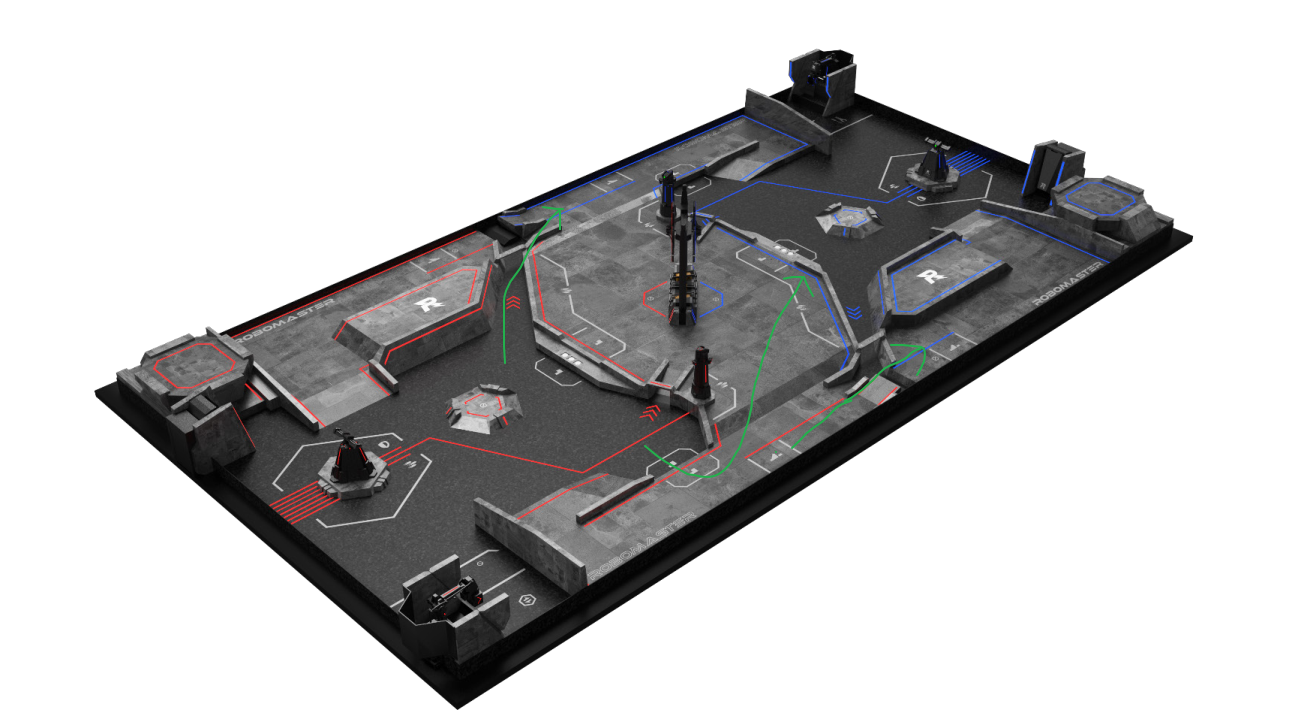
\includegraphics[height=0.35\textwidth]{figure/infantry_tactics.png}
            \hspace{0.5em}
            \label{fig:infantry_tactics}
        \end{figure}
    
    \paragraph{功能需求分析}

    \LTXtable{\textwidth}{Infantry/2.3_functionalRequirement_analysis.tex}
    
    \paragraph{改进方向}

    \LTXtable{\textwidth}{Infantry/2.3_improvementDirection.tex}

    \paragraph{研发进度安排}

    \LTXtable{\textwidth}{Infantry/2.3_developmentSchedule.tex}

    \paragraph{项目组人员分配}

    \LTXtable{\textwidth}{Infantry/2.3_personalAssignment.tex}
    